\documentclass{scrartcl}
 
\usepackage[utf8]{inputenc}
\usepackage[T1]{fontenc}
\usepackage{lmodern}
\usepackage[pdftex]{graphicx}
\usepackage[ngerman]{babel}
\usepackage{amsmath}
\usepackage{amssymb}
\usepackage{tabularx}
\usepackage{multirow}
\usepackage{amsfonts}
\usepackage{tabto}
\usepackage{mathtools}
\TabPositions{0.1in, 0.4in, 0.6in, 0.8in, 1.0in, 1.2in, 3.4in}

\begin{document}
\begin{LARGE}
Spieltheorie - WiSe 2014/15
\end{LARGE}

\begin{Large}
Übungsblatt 7 - Felix Dosch\\[1.0cm]
\end{Large}

\begin{Large}
Aufgabe 7.1\\[0.0cm]
\end{Large}

Zu zeigen: Ist $u : O \rightarrow \mathbb{R}$ eine Nutzenfunktion, die $\succsim$ repräsentiert, und 
$v : \mathbb{R} \rightarrow \mathbb{R}$ eine streng monoton wachsende Funktion, dann ist $v \circ
u : O \rightarrow \mathbb{R}$ mit $(v \circ u)(x) = v(u(x))$ ebenfalls eine Nutzenfunktion die
$\succsim$ repräsentiert.\\

Beweis:\\

Wir benutzen die Definition streng monoton wachsender Funktionen:

\[
f : A \rightarrow B \text{ ist streng monoton wachsend} \Leftrightarrow \forall a, b \in A : a > b
\Rightarrow f(a) > f(b)  \quad (I)
\]

Also: \\

\[
\forall x, y \in O: x \succsim y \Leftrightarrow u(x) \geq u(y)
\] \\
\[
\text{1. Fall: } u(x) = u(y) \xLeftrightarrow{I} v(u(x)) = v(u(y))  \Rightarrow v(u(x)) \geq v(u(y))
\Leftrightarrow x \succsim y
\]
\[
\text{2. Fall: } u(x) > u(y) \xLeftrightarrow{I} v(u(x)) > v(u(y)) \Rightarrow v(u(x)) \geq v(u(y))
\Leftrightarrow x \succsim y
\] \\

Da $v(u(x)) \geq v(u(y)) \Leftrightarrow v(u(x)) = v(u(y)) \vee v(u(x)) > v(u(y))$ und beide Fälle zum
gleichen Ergebnis führen, ist $v(u(x))$ ebenfalls eine Nutzenfunktion, die $\succsim$ repräsentiert. \\

\begin{Large}
Aufgabe 7.2\\[0.0cm]
\end{Large}

a) \\

Vollständigkeit: \\

\[
\forall x, y \in [0,1] \times [0,1] : x \succsim_{L} y \vee y \succsim_{L} x
\]

\begin{itemize}
\item{1. Fall: $x_1 > y_1 \Rightarrow x \succsim_{L} y$}
\item{2. Fall: $y_1 > x_1 \Rightarrow y \succsim_{L} x$}
\item{3. Fall: $x_1 = y_1 \wedge x_2 \geq y_2 \Rightarrow x \succsim_{L} y$}
\item{4. Fall: $x_1 = y_1 \wedge y_2 > x_2 \Rightarrow y \succsim_{L} x$}
\end{itemize}

Reflexivität: \\

\[
\forall x \in [0,1] \times [0,1] : x \succsim_{L} x
\]

$x_1 = x_1 \wedge x_2 \geq x_2 \Rightarrow x \succsim_{L} x$ \\

Transitivität: \\

\[
\forall x, y, z \in [0,1] \times [0,1] : x \succsim_{L} y \wedge y \succsim_{L} z \Rightarrow
x \succsim_{L} z
\]

\begin{itemize}
\item{1. Fall: $x_1 > y_1 \Rightarrow x_1 > y_1 \geq z_1 \Rightarrow x_1 > z_1 \Rightarrow
x \succsim_{L} z$}
\item{2. Fall: $x_1 = y_1 \Rightarrow x_1 = y_1 \geq z_1$}
\begin{itemize}
\item{Unterfall i: $x_1 = y_1 > z_1 \Rightarrow x_1 > z_1 \Rightarrow x \succsim_{L} z$}
\item{Unterfall ii: $x_1 = y_1 = z_1 \Rightarrow x_2 \geq y_2 \geq z_2 \Rightarrow x_1 = z_1
\wedge x_2 \geq z_2 \Rightarrow x \succsim_{L} z$}
\end{itemize}
\end{itemize}

b) Zu Zeigen: Es gibt keine Nutzenfunktion, die die lexikographische Sortierung $\succsim_{L}$
auf $[0,1] \times [0,1]$ repräsentiert. \\

Beweis durch Widerspruch: Angenommen, es gäbe eine solche Nutzenfunktion $f$ und sei $I_a$ das
Intervall $[Inf f(a,R), Sup f(a,R)]$, wobei wir also bei $f(a,R)$ die Menge von Funktionswerten
meinen für festes $a$ in der ersten Komponente und alle möglichen Werte in der zweiten
Komponente. \\

Da $[0,1]$ nicht leer und für jedes $(a, x) \neq (a, y)$ gilt $f(a,x) \neq f(a,y)$ ist das
Intervall $[Inf f(a,R), Sup f(a,R)]$ nicht degeneriert, d.h. das Intervall umfasst nicht nur eine
reelle Zahl. Damit ist insbesondere $|Inf f(a,R) - Sup f(a,R)| \neq 0$ (I). \\

Ausserdem gilt für $a \neq a'$, dass $I_a \cap I_{a'} = \emptyset$, da z.B. für $a > a'$ gilt
$Inf f(a,R) > Sup f(a',R)$ (alle Funktionswerte für einen Wert $a > a'$ in der ersten Komponente
liegen per Definition oberhalb der Funktionswerte für $a'$ in der ersten Komponente). \\

Es kann also eine 1:1-Verbindung zwischen Werten $a \in [0,1]$ und den paarweise disjunkten 
Intervallen $I_a$ hergestellt werden. Betrachten wir nun für alle $a$ den Wert $\epsilon_a =
Sup f(a,R) - Inf f(a,R) \neq 0$ und wählen davon das Minumum $e = min \{\epsilon_a =
Sup f(a,R) - Inf f(a,R)\}$. Die Vereinigung der disjunkten Intervalle bildet das Intervall
$[Inf f(0, R), Sup f(1,R)]$, woraus wir $E = Sup f(1,R) - Inf f(0,R)$ berechnen können. \\

Aus $e$ und $E$ können wir folgern, dass die Anzahl der disjunkten, abgeschlossenen Intervalle
höchstens $\frac{E}{e}$ sein kann, also abzählbar viele. Da nun $[0, 1]$ überabzählbar
ist, die Anzahl der Intervalle jedoch abzählbar, gibt es hier einen Widerspruch (es kann keine
1:1-Korrespondenz zwischen $a$ und $I_a$ geben), also existiert keine Nutzenfunktion $f$, welche
die lexikographische Sortierung repräsentiert. \\

\begin{Large}
Aufgabe 7.3\\[0.0cm]
\end{Large}

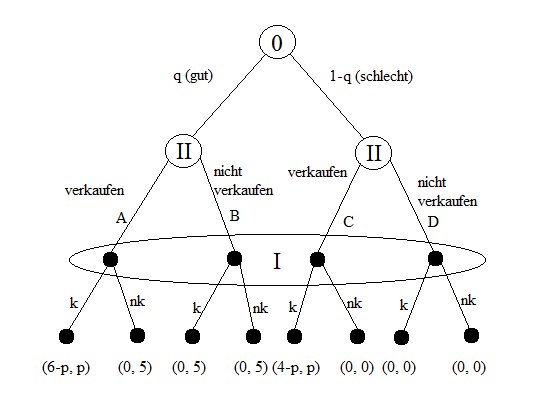
\includegraphics{3_tree.png}

\begin{tabularx}{1\textwidth} {|X|X|X|X|X|}
\hline
$\downarrow$ I / II $\rightarrow$	& $(A, C)$	& $(A, D)$	& $(B, C))$	& $(B, D)$	\\
\hline
kaufen						& $(q \cdot(6-p) + (1-q) \cdot (4-p), p)$	& $(q \cdot (6-p),
q \cdot p)$	& $((1-q) \cdot (4-p),5 \cdot q + (1-q) \cdot p)$	& $(0, 5 \cdot q)$\\
\hline
nicht kaufen	& $(0,5 \cdot q)$	& $(0,5 \cdot q)$	& $(0,5 \cdot q)$ & $(0,5 \cdot q)$\\
\hline
\end{tabularx} \\

Das Spiel ist also:

$H = (N, (T_i)_{i \in N}, p, S, (s_t)_{t \in \times_{i \in N}T_i})$ mit

\begin{itemize}
\item{$N = \{I, II\}$}
\item{$T_I = \{t\}$}
\item{$T_{II} = \{g, s\}$, wobei $g$ = gutes Auto und $s$ = schlechtes Auto}
\item{$p(t, g) = q, p(t, s) = 1 - q$}
\item{$S$ : Menge der Zustände, entspricht Zeilen-/Spaltenkombinationen der Tabelle, wobei Nutzen
$u$ den Tabelleneinträgen entspricht}
\item{$s_t = \{s_{(t, g)}, s_{(t, s)}\}$ : Die Menge der beiden Teilbäume mit Spieler II als Wurzelknoten}
\end{itemize}




\end{document}